\documentclass[11pt,a4paper]{article}
\usepackage[T1]{fontenc}
\usepackage[utf8]{inputenc}
\usepackage{lmodern}
\usepackage{amsmath,amssymb,amsthm,mathtools,mathrsfs}
\usepackage{graphicx,float,xcolor,multicol}
\usepackage[shortlabels]{enumitem}
\usepackage[margin=27mm]{geometry}
\usepackage{microtype,needspace,placeins}
\usepackage{tikz,tikz-cd}
\usetikzlibrary{arrows.meta,calc,positioning,patterns,decorations.pathreplacing}
\usepackage[colorlinks=true,linkcolor=teal,urlcolor=teal,citecolor=teal]{hyperref}
\setlength{\parindent}{0pt}
\setlength{\parskip}{.6em}
\setcounter{secnumdepth}{0}
\allowdisplaybreaks
\raggedbottom
\providecommand{\cross}{\times}
\DeclareUnicodeCharacter{2020}{\ensuremath{\dagger}}
\DeclareMathOperator{\supp}{supp}
\DeclareMathOperator*{\esssup}{ess\,sup}
\providecommand{\chapter}{\section}
\newenvironment{tool}[2]{\subsection*{Tool #1 --- #2}}{}
\newcommand{\ToolRef}[1]{Tool #1}
\newcommand{\FigureTag}[2]{\textit{Figure #1}}
\newcommand{\Result}[1]{\subsection*{#1}}
\newcommand{\Application}[1]{\subsubsection*{Application\if\relax\detokenize{#1}\relax\else\space--- #1\fi}}
\newcommand{\ProofHeading}{\par\textit{Proof.}\space}
\newcommand{\ProofOf}[1]{\par\textit{Proof of #1.}\space}
\newcommand{\RemarkHeading}{\par\textbf{Remark.}\space}
\newcommand{\NoteHeading}{\par\textbf{Note.}\space}
\newcommand{\ExerciseHeading}{\par\textbf{Exercise.}\space}

% Rendering support only; mathematical text is in each independent post.
\usepackage{booktabs,array,longtable}
\definecolor{HandoutBlue}{HTML}{2F6690}
\definecolor{HandoutNavy}{HTML}{17365D}
\newtheorem{theorem}{Theorem}
\newtheorem{lemma}[theorem]{Lemma}
\newtheorem{proposition}[theorem]{Proposition}
\newtheorem{corollary}[theorem]{Corollary}
\newtheorem{conjecture}[theorem]{Conjecture}
\newtheorem{definition}{Definition}
\newtheorem{example}{Example}
\newtheorem{namedtoolcounter}{Tool}
\newenvironment{namedtool}[1]{\begin{namedtoolcounter}[#1]}{\end{namedtoolcounter}}
\newtheorem*{claim}{Claim}
\newtheorem*{remark}{Remark}
\newtheorem*{exercise}{Exercise}
\newtheorem*{question}{Question}
\newtheorem*{observation}{Observation}
\newcommand{\SourceChapter}[2]{\section*{#2}}
\newcommand{\Lecture}[2]{\section*{Lecture #1: #2}}
\newcommand{\unclear}[1]{\textit{[unclear: #1]}}
\newcommand{\sourcegap}{\textit{[unfinished in the source]}}
\DeclareMathOperator{\dist}{dist}
\DeclareMathOperator{\id}{id}
\DeclareMathOperator{\Hol}{Hol}
\DeclareMathOperator{\Per}{Per}
\DeclareMathOperator{\Fix}{Fix}
\DeclareMathOperator{\diam}{diam}
\DeclareMathOperator{\Var}{Var}
\DeclareMathOperator{\Leb}{Leb}
\DeclareMathOperator{\Hom}{Hom}
\DeclareMathOperator{\End}{End}
\DeclareMathOperator{\Ann}{Ann}
\DeclareMathOperator{\Spec}{Spec}
\DeclareMathOperator{\Max}{Max}
\DeclareMathOperator{\Ob}{Ob}
\DeclareMathOperator{\Tor}{Tor}
\DeclareMathOperator{\Ass}{Ass}
\DeclareMathOperator{\Mor}{Mor}
\DeclareMathOperator{\Fun}{Fun}
\DeclareMathOperator{\Nat}{Nat}
\DeclareMathOperator{\Cone}{Cone}
\DeclareMathOperator{\MCG}{MCG}
\DeclareMathOperator{\Aut}{Aut}
\DeclareMathOperator{\Deck}{Deck}
\DeclareMathOperator{\SL}{SL}
\DeclareMathOperator{\PSL}{PSL}
\DeclareMathOperator{\Area}{Area}
\DeclareMathOperator{\im}{im}
\DeclareMathOperator{\PSh}{PSh}
\newcommand{\CRing}{\mathsf{CRings}}
\newcommand{\AMod}{A\text{-}\mathsf{Mod}}
\newcommand{\Ab}{\mathsf{Ab}}
\newcommand{\Z}{\mathbb Z}
\newcommand{\Q}{\mathbb Q}
\newcommand{\R}{\mathbb R}
\newcommand{\C}{\mathbb C}
\newcommand{\N}{\mathbb N}
\newcommand{\kk}{\mathbb k}
\renewcommand{\aa}{\mathfrak a}
\newcommand{\bb}{\mathfrak b}
\newcommand{\pp}{\mathfrak p}
\newcommand{\qq}{\mathfrak q}
\newcommand{\mm}{\mathfrak m}
\newcommand{\nn}{\mathfrak n}
\newcommand{\rad}{\mathrm r}
\newcommand{\cat}[1]{\mathsf{#1}}
\setcounter{secnumdepth}{0}
\allowdisplaybreaks

\graphicspath{{figures/complex-dynamics-notes/}}
\begin{document}
\section*{Hyperbolic Geometry}
% BLOG-CONTENT-BEGIN
We quickly review some preliminaries essential for complex dynamics by answering questions:
\begin{enumerate}
\setcounter{enumi}{0}\item What are hyperbolic surfaces?
\setcounter{enumi}{1}\item Why care about them?
\setcounter{enumi}{2}\item What is so special about them?
\end{enumerate}
\setcounter{theorem}{25}\begin{theorem}[Uniformisation]
Every simply connected Riemann surface is conformally isomorphic to one of
$\widehat{\mathbb C}$ (spherical), $\mathbb C$ (Euclidean), or $\mathbb H\cong\mathbb D$ (hyperbolic).
\end{theorem}
Thus a hyperbolic surface is a Riemann surface whose universal cover is $\mathbb D$. We want to make it a Riemannian manifold in a way that preserves its Riemann-surface automorphisms. Start with $\mathbb D$ or $\mathbb H$, which differ by a Cayley transform.
\setcounter{theorem}{26}\begin{theorem}[Poincar\'e metric on $\mathbb H$]\label{cd7:poincare}
Up to multiplication by a constant, there is a unique Riemannian metric on $\mathbb H$ invariant under every element of $\operatorname{Aut}(\mathbb H)$.
\end{theorem}
% Source page 3
A symmetric Riemannian metric has the form
$g_{11}\,dx\otimes dx+2g_{12}\,dx\otimes dy+g_{22}\,dy\otimes dy$.
For a conformal map $f=u+iv$, taking the $(dx,dy)$ tangent plane to the $(du,dv)$ tangent plane,
\[
du=u_x\,dx+u_y\,dy,\qquad dv=v_x\,dx+v_y\,dy,
\qquad
\begin{pmatrix}du\\dv\end{pmatrix}
=\begin{pmatrix}u_x&u_y\\v_x&v_y\end{pmatrix}\begin{pmatrix}dx\\dy\end{pmatrix}.
\]
This is the differential $df$ in these coordinates. Hence
\begin{align*}
du\otimes du+dv\otimes dv
={}&(u_x^2+v_x^2)\,dx\otimes dx
+2(u_xu_y+v_xv_y)\,dx\otimes dy\\
&+(u_y^2+v_y^2)\,dy\otimes dy.
\end{align*}
Conformality gives $u_xu_y+v_xv_y=0$ and $u_x^2+v_x^2=u_y^2+v_y^2$, motivating the following definition.
% Source page 4
\setcounter{definition}{17}\begin{definition}[Conformal metric]
A metric $ds^2=g_{11}dx^2+2g_{12}dx\,dy+g_{22}dy^2$, where $ds^2$ denotes $ds\otimes ds$, is conformal if $g_{11}=g_{22}$ and $g_{12}=0$.
\end{definition}

Let $S$ be hyperbolic, with universal cover $P\colon\mathbb D\to S$. For $y\in S$, let $U_y$ be evenly covered. Choose $V_a\subset\mathbb D$ so that $P|_{V_a}\colon V_a\to U_y$ is biholomorphic, and set
\[
\gamma_a(P|_{V_a}(z))=\frac{\rho(z)}{|P'(z)|},
\]
where $\rho(z)|dz|$ is the Poincar\'e metric on $\mathbb D$. Let $\{\psi_y\}_y$ be a partition of unity subordinate to
% Source page 6
$\{U_y\}_{y\in S}$. Patch by setting
\[
g=ds^2=\sum_y\psi_y\bigl(\gamma_a(P|_{V_a}(z))\bigr)^2(dx^2+dy^2).
\]

This metric defines distances. For a smooth or piecewise smooth path $p\colon[0,1]\to S$,
\[
\operatorname{length}(p)=\int_pds=\int_0^1|p'(t)|\,dt,
\qquad |p'(t)|=\sqrt{ds\otimes ds(p'(t),p'(t))}.
\]
The formula for smooth paths extends in the same way to piecewise smooth paths.
\setcounter{definition}{18}\begin{definition}[Poincar\'e distance]
For $z_0,z_1\in S$, let $\mathcal Z$ be the smooth or piecewise smooth paths joining them. Define $\dist_S(z_0,z_1)=\inf_{p\in\mathcal Z}\operatorname{length}(p)$.
\end{definition}
% Source page 7
\setcounter{theorem}{27}\begin{lemma}[Completeness]\label{cd7:complete}
The space $(S,\dist_S)$ is complete. Given any $z_0,z_1\in S$, there is a path $p$ with $\operatorname{length}(p)=\dist_S(z_0,z_1)$; in other words, there is at least one geodesic.
\end{lemma}
\begin{remark}
Heine--Borel holds for hyperbolic spaces: $N_r(z_0)=\{z\in S:\dist_S(z,z_0)\le r\}$ is compact for every $r>0$.
\end{remark}
An explicit geodesic construction is sketched below. Let $B$ be a ball of local isometry about $z_0$, and choose a path $p$ to $z_1$ with $\operatorname{length}(p)=\dist(z_0,z_1)+\varepsilon$, possible by the definition of infimum.
\begin{figure}[H]\centering
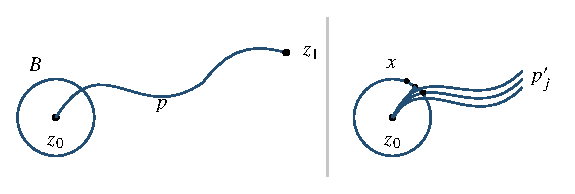
\includegraphics[width=.85\textwidth]{cd7-fig-03.pdf}
\FigureTag{CD7.3}{fig:cd7-03}
\end{figure}
Consider paths $p_j'$ with lengths $\dist(z_0,z_1)+\varepsilon_j'$, where $\varepsilon_j'\le\varepsilon$ and $\varepsilon_j'\to0$. If they cross $\partial B$ at $x_j$, choose an accumulation point $x$. Join $z_0$ to $x$ by a geodesic, then repeat.
% Source page 9
We care about hyperbolic surfaces because the other surfaces are well known: $\widehat{\mathbb C}$, $\mathbb C$, $S^1\times S^1$, and $S^1\times\mathbb R$. This follows by checking fixed-point-free automorphisms of $\widehat{\mathbb C}$ and discrete subgroups of $\operatorname{Aut}(\mathbb C)$; their quotients give all spherical and Euclidean surfaces. They all have abelian fundamental group. Thus a surface with nonabelian fundamental group is immediately hyperbolic: hyperbolic surfaces abound.
\setcounter{theorem}{28}\begin{lemma}\label{cd7:three-punctures}
The surface $\widehat{\mathbb C}\setminus\{p,q,r\}$ is hyperbolic.
\end{lemma}
\begin{proof}
It is a Riemann surface with nonabelian fundamental group:
$\pi_1(\widehat{\mathbb C}\setminus\{p,q,r\})\cong\pi_1(\mathbb C\setminus\{p,q\})\cong\mathbb Z*\mathbb Z$.
\end{proof}
\setcounter{theorem}{29}\begin{corollary}[Picard's theorem]
If a holomorphic map $f\colon\mathbb C\to\mathbb C$ omits two distinct values, it is constant.
\end{corollary}
\begin{proof}
If $f$ omits $a,b$, it maps $\mathbb C$ to the hyperbolic surface $\mathbb C\setminus\{a,b\}$. It lifts to $\widetilde f\colon\mathbb C\to\mathbb D$.
\begin{figure}[H]\centering
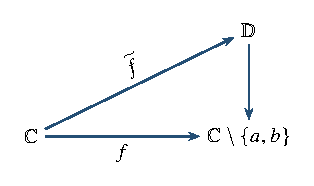
\includegraphics[width=.40\textwidth]{cd7-fig-04.pdf}
\FigureTag{CD7.4}{fig:cd7-04}
\end{figure}
Liouville's theorem makes $\widetilde f$ constant. Here we regard $\mathbb D\subset\mathbb C$ without giving it its Poincar\'e metric.
\end{proof}
% Source page 10
In fact, hyperbolic surfaces are embedded as submanifolds in every Riemann surface. If $\mathbb C$ or $\widehat{\mathbb C}$ covers $S$, it only remains to consider the cylinder and torus. Removing one point there removes infinitely many points in $\mathbb C$; the resulting cover sits in $\mathbb C\setminus\{p,q\}$, or in $\widehat{\mathbb C}\setminus\{p,q,r\}$.

% Source page 12
% BLOG-CONTENT-END
\end{document}
